\documentclass[UTF8]{ctexart}
\title{猫站小报 第 2 期}
\author{猫站小报编辑部}
\date{\today}
\usepackage{indentfirst}
\setlength{\parindent}{2em}
\usepackage{ulem}
\usepackage{xcolor}
\usepackage{graphicx}
\usepackage{geometry}
\geometry{left=0.2in,right=0.2in,top=0.2in,bottom=0.2in}
\usepackage{listings}

\begin{document}
\maketitle
\part{编辑部专版}
\section{以猫站为反面教材谈如何设计安全的网站}
网络安全是每一位网站运营者必须要考虑的事情。而猫站的网络安全建设不能说十分坚固,只能说是完全没有。今天我们就以猫站为一个反面案例来教想要运营自己的网站的同学如何做好网络安全建设。
\subsection{XSS注入攻击防护}
如果你的网站需要在页面中动态插入HTML,一定要做好XSS注入攻击防护。XSS攻击,即跨站脚本攻击,它的核心原理就是在网页中注入恶意脚本。在猫站,你可以随意在帖子里面写JS脚本,当用户加载到这个帖子的时候,JS脚本就会被执行。例如一条评论的内容是:
\begin{lstlisting}[language=HTML]
<img src="static/..." onload="alert(‘哇袄!’)">
\end{lstlisting}
那么,当浏览者加载这个图片的时候,就会执行onload中的脚本,浏览器就会弹出弹窗:哇袄!

对于这种攻击方式,只需要对用户输入的所有特殊字符使用转义字符替换就能完全防下来。例如把所有用户输入的<替换为\&lt;破坏HTML结构,浏览器就不会执行XSS注入攻击的脚本。如果是是富文本输入,可以使用DOMPurify这样的npm安全库来清洗掉用户输入中的带XSS脚本的的HTML。当然,网站的前端要做防XSS校验,网站的后端也要做XSS校验。如果黑客得到了你的API地址,又拿到了Token,你的后端又没有做XSS校验,就能绕开前端的XSS校验,把带有恶意攻击脚本的HTML内容插入进你的数据库中。

\subsection{后端API鉴权}
对于一些敏感的API,一定要做足鉴权,如果权限不足,就返回401 Unauthorized状态码,阻止权限不足的黑客获取敏感信息。但猫站几乎所有的API都没有鉴权,导致黑客可以随意查询举报记录。

现代网站常用JWT来进行鉴权,在用户登录后,返回一个Token,并把Token存储在浏览器Cookie中。JWT分为三部分:Header,Payload,Signature。Header会指定Token使用的算法,和token类型。Payload存放了实际需要的数据,用户可以自定义内容,如用户身份信息。Signature中是服务器对前两个部分用Header中指定的算法进行的签名。这个签名是用来验证这个Token是否为服务器签发的,如果验证得到这个Token确实是服务器签发的,就根据Payload中的信息,决定是否要把该敏感信息返回给用户。注意,不要在payload里存放任何敏感信息,例如密码。

\subsection{增加更多的CAPTCHA}
CAPCHAT,俗称验证码,是用来防机器人和爬虫的。由于猫站几乎没有任何的CAPTCHA,导致机器人可以批量注册账号,大量刷屏。对于任何关于数据库操作的请求,最好都加上验证码,可以提高黑客制造机器人刷屏的的成本。
\subsection{双因素验证}
对于登录相关的行为,最好加上双因素认证,常见的认证方式有短信验证码和TOTP验证码。这样可以提高登录时的安全性,有效防止盗号的发生。例如洛谷引入了TOTP验证码,有效防止了机房惨案的发生。\sout{PyPI的验证码成功把我堵在了外面}
\pagebreak

\part{积木纪元}
\subsection{时之流逝 : 回归}

\includegraphics[width=0.4\textwidth]{assets/02/kitten-1.png}

\noindent
\textbf{作者:} 虚数\\
\textbf{ID:} 273015666\\
\textbf{介绍:}一个用Kitten实现的3D作品,根据虚数给编辑透露出的代码片段,他几乎用kitten手搓了一个OpenGL实现。此作品尚未完成,但值得所有人的点赞鼓励 \\
\textbf{编辑评:}编辑是调包侠,没资格评价造轮子的大佬的作品
\hfill
\includegraphics[width=0.08\columnwidth]{assets/02/kitten-1-qrc.png}
\subsection{火柴人你瞅啥}
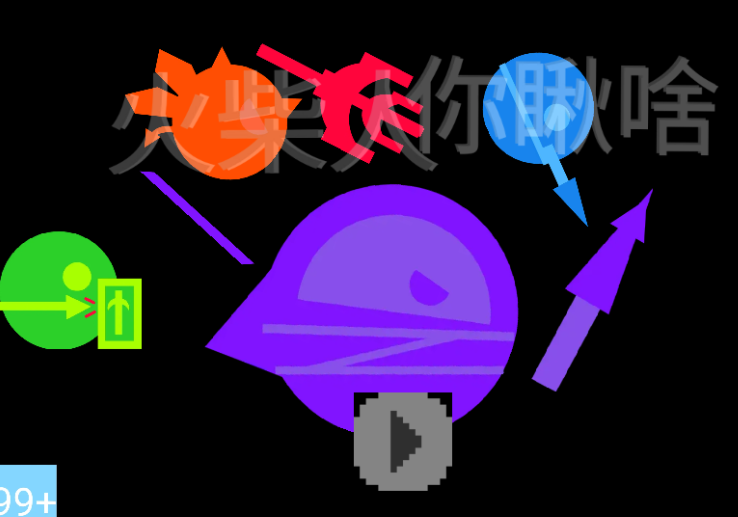
\includegraphics[width=0.4\textwidth]{assets/02/kitten-2.png}

\noindent
\textbf{作者:}雨果猫 \\
\textbf{ID:}266291679 \\
\textbf{介绍:}一个使用Nemo制作的小游戏,完成度相当高\\
\textbf{编辑评:}其实更适合用手机玩,有些要素确实很像广告里的小游戏(
\hfill
\includegraphics[width=0.08\columnwidth]{assets/02/kitten-2-qrc.png}

\pagebreak
\part{代码诗篇}
\subsection{未知}
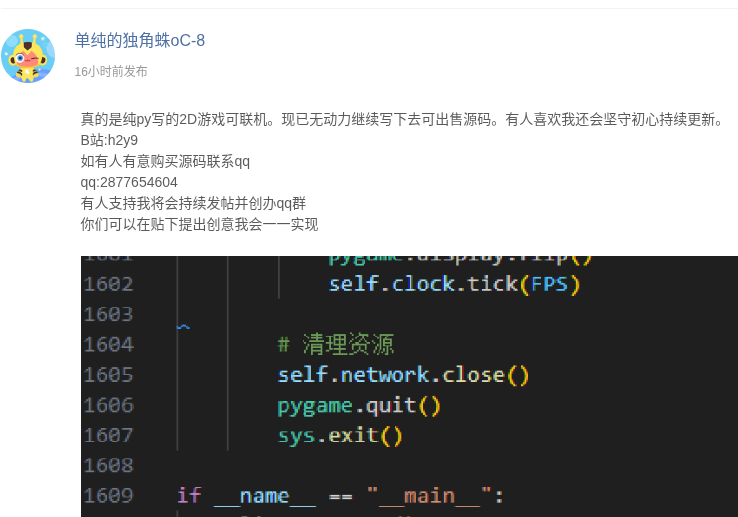
\includegraphics[width=0.5\textwidth]{assets/02/python-1.png}

\noindent
\textbf{作者:} 单纯的独角蛛oC-8\\
\textbf{链接:}https://shequ.codemao.cn/community/1634470 \\
\textbf{介绍:}这是一个快要弃坑的闭源作品,根据作者所放出的图,代码量有一千余行\\
\textbf{编辑评:}我更希望能借这个小平台给作者注入一些热情
\hfill 
\includegraphics[width=0.08\columnwidth]{assets/02/python-1-qrc.png}

\subsection{原神抽卡模拟器}
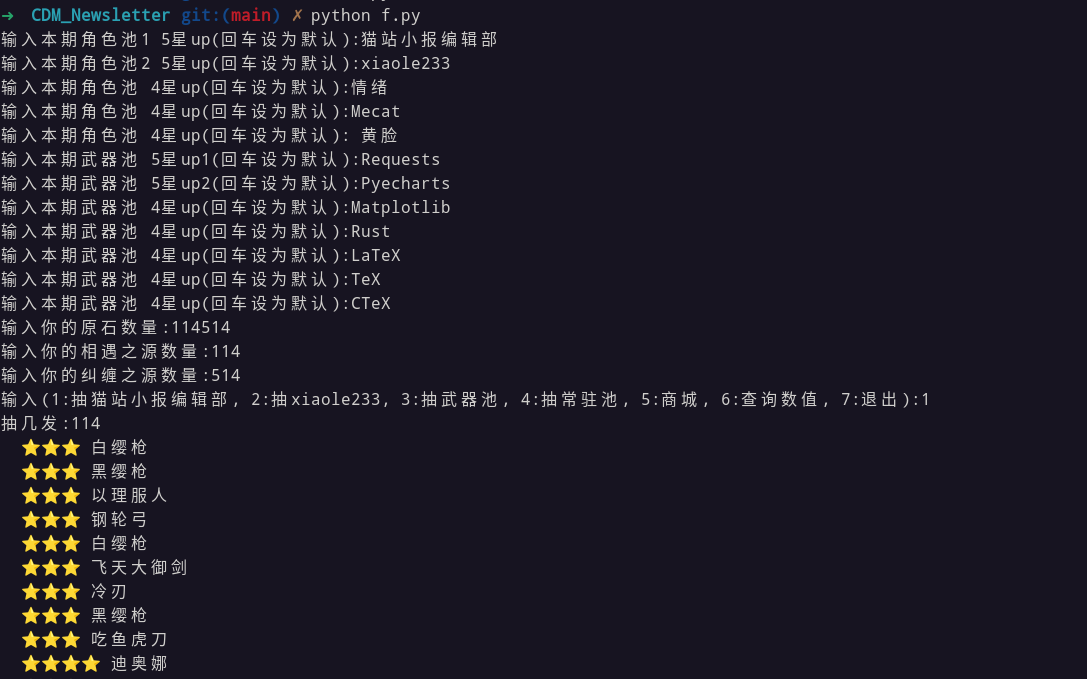
\includegraphics[width=0.6\textwidth]{assets/02/python-2.png}

\noindent
\textbf{作者:}不知名的原神玩家 \\
\textbf{链接:}https://shequ.codemao.cn/community/1632113 \\
\textbf{介绍:}一个用Python写的原神抽卡模拟器,代码量1000多行\footnotemark\\
\textbf{编辑评:}编辑部已放弃重构,Black代码格式化都跑崩了(
\hfill 
\includegraphics[width=0.08\columnwidth]{assets/02/python-2-qrc.png}
\footnotetext{源代码存在错误,修正后放在了编辑的Github上,后记中自取}
\pagebreak
\part{传火者}
\begin{center}
	\zihao{-1}
	\textbf{Python中的Lambda表达式}
	\normalsize
	供稿:xiaole233
\end{center}
在Python中,我们常用def关键字来定义函数,像是这样
\begin{lstlisting}[language=python]
def add(a,b):
	return a+b;
\end{lstlisting}
但你知道吗,除了用def,还有另一种方式来定义函数,这就是lambda表达式,以下是一个lambda表达式的示例
\begin{lstlisting}[language=python]
add=lambda a,b:a+b
print(add(1,2))
\end{lstlisting}
lambda表达式本质上是一种匿名函数,他可以防止简单的函数造成命名空间污染,当然,你也可以把这个匿名函数赋值给一个变量从而让这个函数具有名称。lambda仅支持单行表达式,适合短期使用的简单逻辑。它的基本语法是:
\begin{lstlisting}
lambda 参数列表:返回值表达式
\end{lstlisting}
lambda常用于转换数据,自定义排序规则,动态生成函数,条件逻辑封装和GUI的事件处理,这些环境下使用lambda可以大大节约代码量,提高可读性。

\textbf{请注意!}对于需要复用的代码,不要使用lambda,不要把复杂的逻辑写到lambda表达式里面,也不要尝试嵌套lambda表达式,这样会让你的代码可读性大大降低。

总结一点,lambda并不是要取代def,而是要简化def,使用lambda,请遵循以下原则:
\begin{itemize}
	\item 逻辑能用20秒理解,用lambda代替def
	\item 操作集中在单行的表达式中,用lambda代替def
	\item 你要定义的函数名没有意义,用lambda代替def
\end{itemize}
\pagebreak
\part{撤硕儿}
\begin{center}
\textbf{该板块为第2期新增,主要是编辑部和猫舍成员对社区某些帖子的吐槽,来满足各位的吃屎欲望}
\end{center}
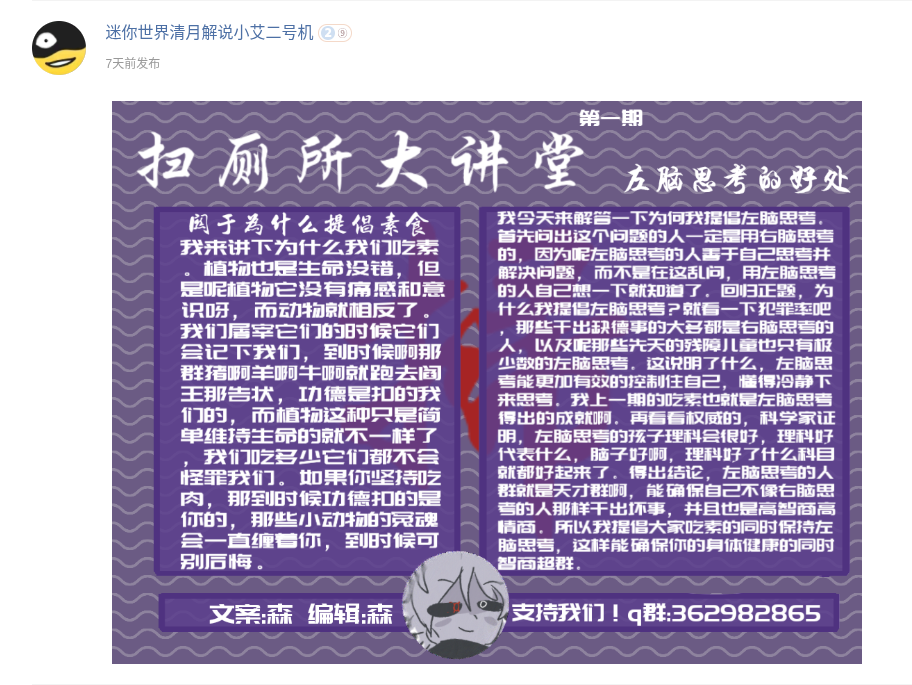
\includegraphics[width=0.8\textwidth]{assets/02/toliet-1.png} \\
\textbf{编辑评}:左脑思考素食,右脑思考左脑(图片的左右顺序)

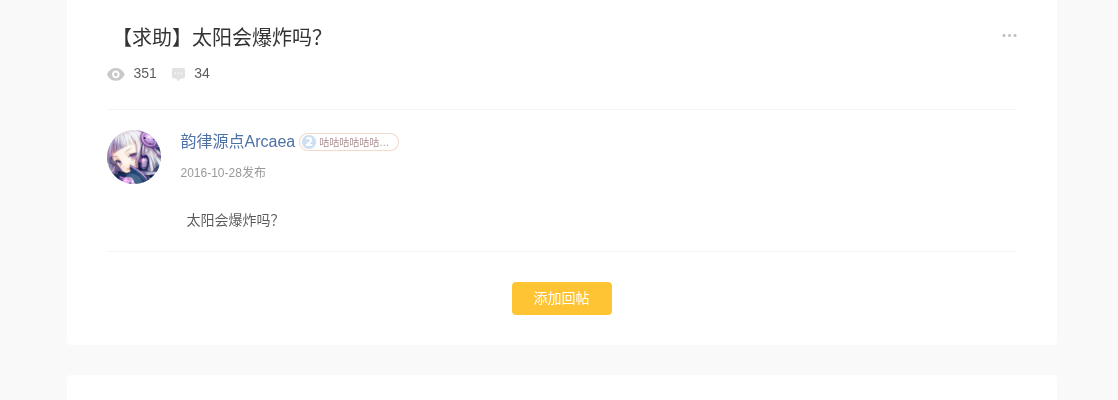
\includegraphics[width=0.8\textwidth]{assets/02/toliet-2.png} \\
\textbf{编辑评}:来考古

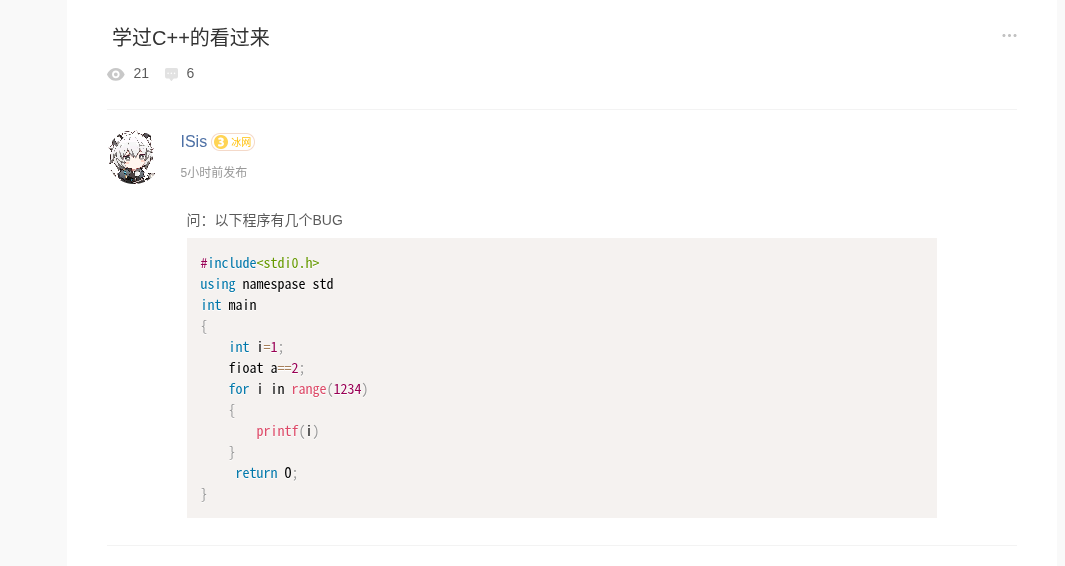
\includegraphics[width=0.8\textwidth]{assets/02/toliet-3.png} \\
\textbf{编辑评}:万一这是C- -呢(

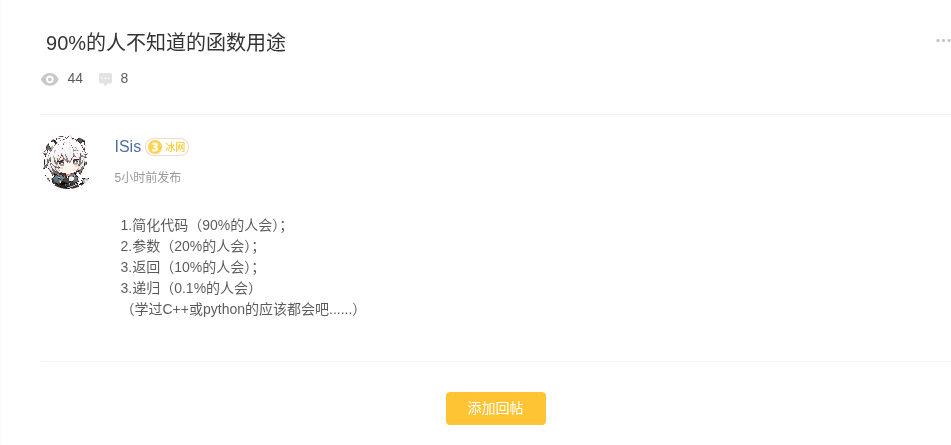
\includegraphics[width=0.8\textwidth\\]{assets/02/toliet-4.png} \\
\textbf{虚数}:坏了我都会
\pagebreak
\part{后记}
\paragraph{编辑} 目前唯一编辑也是主笔:xiaole233 邮箱地址:xiao\_2010@outlook.com
\paragraph{感谢截至到\today 支持小报的读者们,排名不分先后:}
\begin{center}虚数、悠​闲​的​阿​米​巴​、Mecat、荔枝xi、小刘12345678、编程追梦者、无敌版滑稽战神
\end{center}
\paragraph{版权说明} 
猫站小报 © 2025 by 小报编辑部 is licensed under CC BY 4.0.\\ To view a copy of this license, visit https://creativecommons.org/licenses/by/4.0/ \\
\begin{center}
\begin{figure}[htbp]
	\centering
	
\includegraphics[width=0.1\textwidth]{assets/02/yuanshen-qrc.png}
	\caption{原神抽卡模拟器源码}
\end{figure}
\begin{figure}[htbp]
	\centering
	
\includegraphics[width=0.1\textwidth]{assets/repo-qrc.png}
	\caption{小报的Github仓库}
\end{figure}
\end{center}
	

\end{document}